\documentclass[11pt,oneside,a4paper]{article}
\usepackage[utf8]{inputenc}
\date{}
\usepackage[linesnumbered,ruled,vlined]{algorithm2e}
\SetKwInput{KwInput}{Input}                % Set the Input
\SetKwInput{KwOutput}{Output}              % set the Output<z
\usepackage{blindtext}
\usepackage{changepage}


\usepackage[formats]{listings}  %% Code listing%% Code format

%\usemintedstyle{friendly}
\usepackage{amsmath}
\usepackage{color}
\usepackage{tcolorbox}
\usepackage{sectsty}
\usepackage{stmaryrd}
\usepackage{gensymb}
\usepackage{tikz}
\usetikzlibrary{shapes,snakes}
\usepackage{wasysym}
\usepackage{amsfonts}
\usepackage{xcolor}
\usepackage{graphicx}
\usepackage{stmaryrd}
\usepackage{mathtools}
\usepackage{amsthm}
\usepackage{caption}
\usepackage{subcaption}
\usepackage[margin=1.2in]{geometry}
%__________WIDE HAT_________
\usepackage{scalerel,stackengine}
\stackMath
\newcommand\reallywidehat[1]{%
\savestack{\tmpbox}{\stretchto{%
  \scaleto{%
    \scalerel*[\widthof{\ensuremath{#1}}]{\kern-.6pt\bigwedge\kern-.6pt}%
    {\rule[-\textheight/2]{1ex}{\textheight}}%WIDTH-LIMITED BIG WEDGE
  }{\textheight}%
}{0.5ex}}%
\stackon[1pt]{#1}{\tmpbox}%
}
\parskip 1ex
%______________________________
\usepackage{hyperref}
\hypersetup{
    colorlinks=true,
    urlcolor=blue
}
\setlength{\parindent}{0in}
\theoremstyle{definition}
\newtheorem{definition}{Definition}[section]

\theoremstyle{remark}
\newtheorem*{remark}{Remark}
\usepackage{amsmath}
\usepackage[T1]{fontenc}
\usepackage{float}
\usepackage[british,UKenglish,swedish,USenglish,english,american]{babel}
\usepackage[T1]{fontenc}
\usepackage{fancyhdr}
\usepackage{natbib}
%\pagestyle{fancy}
\begin{document}
\renewcommand{\bibname}{References}
\hypersetup{citecolor=black}
\begin{titlepage}\centering
\vspace*{\fill}
\Huge Assignment 2\\
\vspace*{10mm}
\large Includes methods of Directed Graphical Models, Dynamic programming, Variational Inference and Expectation Maximisation \\
\vspace*{\fill}
\large \textsc{DD2434 Advanced Machine Learning} \\
\textsc{Filip Bergentoft, bergento@kth.se} \\
\end{titlepage}

\newpage


\section*{3.3 Complicated likelihood for leaky units on a tree}


Let $u_{1}\downarrow$ and $u_{2}\downarrow$ be the children of node u, then we get the following 


\begin{figure}[H]
\begin{center}
  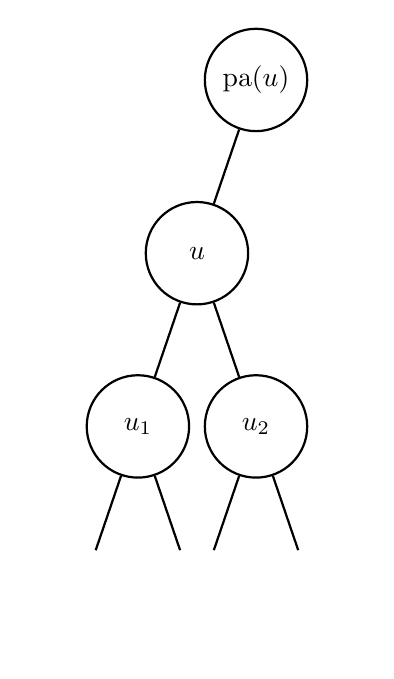
\begin{tikzpicture}[thick, minimum size=1.3cm, level distance=2.2cm]
    \node[circle,draw]{pa$(u)$}
        child { node[circle,draw]{$u$}
            child { node[circle,draw]{$u_1$}
                child { node[circle]{} }
                child { node[circle]{} }
                }
            child { node[circle,draw]{$u_2$}
                child { node[circle]{} }
                child { node[circle]{} }
                }
        }
        child [ missing ];
  \end{tikzpicture}
\end{center}
  \caption{Binary tree starting at parent of $u$, branches below $u_1, u_2$ denotes subtrees}
\end{figure}
Let $p_{Z_{u \downarrow}} = \sum_{Z_{u \downarrow}} p(X_u, X_{u \downarrow}, Z_{u \downarrow}|Z_u, Z_{\text{pa}(u)})$ where $\sum_{Z_{u \downarrow}}$ denotes the summation over all latent variables below $u$, not including $u$, then

\begin{align}
  p_{Z_{u \downarrow}} & = \sum_{Z_{u \downarrow}} p(X_u, X_{u_1}, X_{u_2}, X_{u_1 \downarrow}, X_{u_2 \downarrow}, Z_{u_1 \downarrow}, Z_{u_2 \downarrow}|Z_u, Z_{\text{pa}(u)}, Z_{u_1}, Z_{u_2})p(Z_{u_1}) p(Z_{u_1\downarrow}) \nonumber \\
  & = \sum_{Z_{u \downarrow}} p(X_u|Z_u, Z_{\text{pa}(u)}, Z_{u_1}, Z_{u_2}) p(Z_{u_1})p(Z_{u_2})p(X_{u_1}, X_{u_1\downarrow}, Z_{u_1\downarrow}|Z_{u_1}, Z_u) p(X_{u_2}, X_{u_2\downarrow}, Z_{u_2\downarrow}|Z_{u_2}, Z_u) \nonumber\\
  & = \sum_{Z_{u \downarrow}} \bigg[ p(X_u|Z_u, Z_{\text{pa}(u)}, Z_{u_1}, Z_{u_2})p(Z_{u_1})p(Z_{u_2}) \nonumber\\
  & \qquad\qquad p(X_{u_1}, X_{u_1\downarrow}, Z_{u_1\downarrow}|Z_{u_1}, Z_u) p(X_{u_2}, X_{u_2\downarrow}, Z_{u_2\downarrow}|Z_{u_2}, Z_u) \bigg] \nonumber\\
  & = \sum_{Z_{u_1}, Z_{u_2}} \bigg[ p(X_u|Z_u, Z_{\text{pa}(u)}, Z_{u_1}, Z_{u_2})p(Z_{u_1})p(Z_{u_2}) \nonumber\\
  & \qquad\qquad
  \Big( \sum_{Z_{u_1\downarrow}} p(X_{u_1}, X_{u_1\downarrow}, Z_{u_1\downarrow}|Z_{u_1}, Z_u) \Big)
  \Big( \sum_{Z_{u_2\downarrow}} p(X_{u_2}, X_{u_2\downarrow}, Z_{u_2\downarrow}|Z_{u_2}, Z_u)\Big) \bigg] \nonumber\\
  & = \sum_{Z_{u_1}, Z_{u_2}} \bigg[ p(X_u|Z_u, Z_{\text{pa}(u)}, Z_{u_1}, Z_{u_2})p(Z_{u_1})p(Z_{u_2}) \Big(p_{Z_{u_1\downarrow}}\Big) \Big( p_{Z_{u_2\downarrow}}\Big)\bigg] \nonumber \\
  & = \sum_{Z_{u_1}, Z_{u_2}} \bigg[ \mathcal{N}\Big(X_u|(1-\alpha)\mu_{Z_u} +\frac{\alpha}{3}(\mu_{Z_{u_1}}+\mu_{Z_{u_2}}+\mu_{Z_{\text{pa}(u)}}) \Big) \cdot \nonumber\\
  & \qquad\qquad\qquad  \cdot \pi(Z_{u_1}) \pi(Z_{u_2}) \Big(p_{Z_{u_1\downarrow}}\Big) \Big( p_{Z_{u_2\downarrow}}\Big)\bigg]\nonumber
\end{align}

On a more compact form we have thus shown that

\begin{align}
  p_{Z_{u \downarrow}} & = \sum_{Z_{u \downarrow}} p(X_u, X_{u \downarrow}, Z_{u \downarrow}|Z_u, Z_{\text{pa}(u)}) \\
  & = \sum_{Z_{u_1}, Z_{u_2}} \bigg[ \mathcal{N}\Big(X_u|(1-\alpha)\mu_{Z_u} +\frac{\alpha}{3}(\mu_{Z_{u_1}}+\mu_{Z_{u_2}}+\mu_{Z_{\text{pa}(u)}}) \Big) \cdot \\
  & \qquad\qquad\qquad  \cdot \pi(Z_{u_1}) \pi(Z_{u_2}) \Big(p_{Z_{u_1\downarrow}}\Big) \Big( p_{Z_{u_2\downarrow}}\Big)\bigg]
\end{align}
Which shows the recursion.


We have thus ended up with two new subproblems $p_{Z_{u_1\downarrow}}$ and $p_{Z_{u_2\downarrow}}$ from $p_{Z_{u \downarrow}}$ which can be divided into subproblems continuously until the leaves are reached.
\\

It is important to note that $p_{Z_{u_1\downarrow}}$ is independent of $Z_{u_2}$ and similarly $p_{Z_{u_2\downarrow}}$ is independent of $Z_{u_1}$. It is thus only necessary to compute $p_{Z_{u_1\downarrow}}$ when summing over $Z_{u_1}$. When summing over $Z_{u_2}$ the value for $p_{Z_{u_1\downarrow}}$ can be computed once, stored and then be reused. Applying this for all subproblems results in a linear algorithm for computing $p(X)$.

\subsection*{Special case: root}

Let $u$ denote the root and $u_1, u_2$ denote its children.
\begin{figure}[H]
\begin{center}
  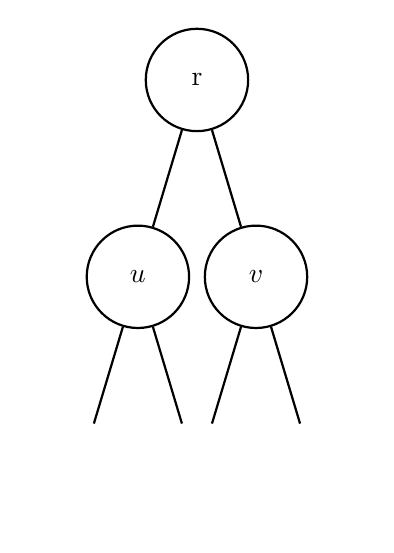
\begin{tikzpicture}[thick, minimum size=1.3cm, level distance=2.5cm]
    \node[circle,draw]{r}
        child { node[circle,draw]{$u$}
            child { node[circle]{}}
            child { node[circle]{}}
        }
        child { node[circle,draw]{$v$}
            child { node[circle]{}}
            child { node[circle]{}}
        };
  \end{tikzpicture}
\end{center}
\caption{Binary tree starting at root r, branches below $u, v$ denotes subtrees}
\end{figure}

\begin{align}
  & p(X) = \sum_{Z_u, Z_{u_1}, Z_{u_2}}\bigg[p(X_u|Z_{u_1}, Z_{u_2}, Z_u) p(Z_{u_1}, Z_{u_2}, Z_u) \nonumber\\
  & \qquad\qquad\quad \Big(\sum_{Z_{u_1 \downarrow}} p(X_{u_1}, X_{u_1 \downarrow}, Z_{u_1 \downarrow}|Z_{u_1}, Z_u) \Big)\Big(\sum_{Z_{u_2 \downarrow}} p(X_{u_2}, X_{u_2 \downarrow}, Z_{u_2 \downarrow}|Z_{u_2}, Z_u) \Big)\bigg] \nonumber \\
  & = \sum_{Z_u, Z_{u_1}, Z_{u_2}}\bigg[\mathcal{N}\Big(X_u|(1-\alpha)\mu_{Z_u} +\frac{\alpha}{2}(\mu_{Z_{u_1}}+\mu_{Z_{u_2}}) \Big) \pi(Z_u) \pi(Z_{u_1}) \pi(Z_{u_2})\\
  & \qquad\qquad\quad \Big(\sum_{Z_{u_1 \downarrow}} p(X_{u_1}, X_{u_1 \downarrow}, Z_{u_1 \downarrow}|Z_{u_1}, Z_u) \Big)\Big(\sum_{Z_{u_2 \downarrow}} p(X_{u_2}, X_{u_2 \downarrow}, Z_{u_2 \downarrow}|Z_{u_2}, Z_u) \Big)\bigg]
\end{align}


\subsection*{Special case: leaf}
Let $u_1$ denote a \textit{leaf node}, it thus has no children which implies that $Z_{u_1 \downarrow} = \emptyset$.

Using previous definition of $p_{Z_{u \downarrow}}$ yields

 \begin{align}
   p_{Z_{u_1 \downarrow}} & = \sum_{Z_{u_1 \downarrow}} p(X_{u_1}, X_{u_1 \downarrow}, Z_{u_1 \downarrow}|Z_{u_1}, Z_{\text{pa}(u_1)}) \nonumber\\
   & = p(X_{u_1}|Z_{u_1}, Z_{\text{pa}(u_1)}) \nonumber\\
   & = \mathcal{N}\Big(X_{u_1} | (1-\alpha)\mu_{Z_{u_1}} + \alpha \mu_{Z_{\text{pa}(u_1)}} \Big)
 \end{align}

\end{document}
